%%%%%%%%%%%%%%%%%%%%%%%%%%%%%%%%%%%%%
%%%%% PHYS305 Assignment 1
%%%%% Zachary Martin
%%%%% 21 January 2019
%%%%%%%%%%%%%%%%%%%%%%%%%%%%%%%%%%%%%

\documentclass[aps,prl,twocolumn,superscriptaddress]{revtex4-1}

% the line above is necessary to start any latex document.
% this is one variation that should work for most things.
% if you want double spaceing, use the following:
%
%\documentclass[prd,preprint,letterpaper]{revtex4}
%
% the "preprint" designation will make a wider line
% spacing, good for markup.

\usepackage{graphicx}  % this is the up-to-date package for all figures
\graphicspath{{pictures/}} 	% Set Graphics Path
\usepackage{siunitx} % Scientific Notation and Units
\usepackage{amsmath, amssymb, gensymb, mathtools, bm} 	% Mathematical Tools
\usepackage{verbatim}  % for the comment environment
\usepackage{color}
% \usepackage{arydshln} % Dashed lines in table

% Shortcut Commands
\newcommand{\paren}[1]{\left( #1 \right)} 	% Parentheses for complicated expressions
\newcommand{\bparen}[1]{\left[ #1 \right]}	% Bracket parentheses for complicated expressions
\newcommand{\cmod}[1]{\left| #1 \right|}	% Mod or Absolute value

\bibliographystyle{apsrev}

% these are some custom control of the page size and margins
% \topmargin= 0.2in  % these 1st two may be needed for some computers
\textheight=9in
\textwidth=6.5in
% these next two lines give us centered text
\oddsidemargin=0cm
\evensidemargin=0cm

\begin{document}

% Title Contents
\title{PHYS 305 Assignment 1: Approximating $\pi$ Using the Leibniz Series and Wallis Formula}
\author{Zachary Martin}
\affiliation{University of Hawaii at Manoa}
\date{23 January 2019}

\begin{abstract}
In this assignment, we explore the Leibniz and Wallis approximations for the value of $\pi$. Using a program written in C++, we computed these series for $N = 1, ..., 10, 100, 1000, 10000$ terms/factors and the percent error of the approximation. We confirm the convergence towards $\pi$ and find that their rates of convergence are extremely slow, implying that a large value of $N$ would be needed to get an accurate value of $\pi$. This directly indicates the importance of computational methods, as evaluating these series by hand would take a incredible amount of time.
\end{abstract}

\maketitle

\section{Introduction and Overview}
We have found that mathematical series have countless applications to physics, from calculating transcendental numbers to approximating functions as polynomials. In the 17th century, Gottfried Wilhelm Leibniz discovered a series that can be used to calculate the value of $\pi$ \cite{Leibniz}. This series arises in solutions to Fourier series in some physical systems. In the same century, John Wallis discovered the Wallis formula, a product series that can also be used to calculate the value of $\pi$. As it turns out, this series comes up when solving the energy states of Hydrogen using a technique called the variational approach \cite{WallisQuantum}. These examples of the connections between mathematical series and physics provide enough reason to explore the nature of these series.

\section{Description of Computational problem}
We want to calculate an approximation for $\pi$ using $N$ terms/factors of each series. Rather than calculating each term by hand, we will create a program using C++ which finds the sum or product of the series of interest after given a user input number of terms/factors. The program should then multiply by the right factor to give the approximation for $\pi$. Then, it should calculate for each given $N$ the percent error of the approximation of $pi$. By plotting the error as a function of $N$, we can find the relationship between the two and analyze the convergence of the series.

\section{Relevant equations}
The first series of interest is the Leibniz series. This series comes from solving the integral of the derivative of $\tan ^{-1} x$ using a Taylor expansion \cite{LeibnizDerivation}. Then letting $x = 1$, we obtain
\begin{equation}
	\frac{\pi}{4} = \sum_{j = 1}^{\infty} \frac{\paren{-1}^{j + 1}}{2 j - 1} ~. \label{eqn:Leibniz}
\end{equation} 

The second series of interest is the Wallis formula, which follows from an infinite product series of $\sin x / x$ \cite{WallisDerivation}. We let $x = \pi / 2$ and obtain
\begin{equation}
	\frac{\pi}{2} = \prod_{j = 1}^{\infty} \frac{\paren{2 j}^2}{\paren{2 j - 1} \paren{2 j + 1}} ~. \label{eqn:Wallis}
\end{equation}
Setting an upper limit $N$ on these series and multiplying by the appropriate factor ($4$ for Equation \ref{eqn:Leibniz} and $2$ for Equation \ref{eqn:Wallis}) then gives an approximation for $\pi$. \\
Then, to calculate the percent error of the approximation, $\bar{\pi}$, from the true value, $\pi$, we use the formula
\begin{equation}
	P_{\text{err}} = \frac{\cmod{\bar{\pi} - \pi}}{\pi} ~. \label{eqn:Perr}
\end{equation}
This should change as a function of $N$ which we will analyze in the next section.

\section{Results and Analysis}

\begin{table}[th] % table environment to enable captions and labels, [h] = 'here'
	\begin{center}
		\begin{tabular*}{\columnwidth}{|@{\extracolsep{\fill}} c | c c c c | }
		\hline
 		$N$ & $\bar{\pi}_L$ & $P_{\text{err, L}}$ & $\bar{\pi}_W$ & $P_{\text{err, W}}$ \\
 		\hline\hline
 		1 & 4 & 27.324 & 2.66667 & 15.1174 \\
 		2 & 2.66667 & 15.117 & 2.84444 & 9.45852 \\
 		3 & 3.46667 & 10.347 & 2.92571 & 6.87162 \\
 		4 & 2.89524 & 7.8417 & 2.97215 & 5.39339 \\
 		5 & 3.33968 & 6.3054 & 3.00218 & 4.43777 \\
 		6 & 2.97605 & 5.2695 & 3.02317 & 3.7695 \\
 		7 & 3.28374 & 4.5246 & 3.03867 & 3.27601 \\
 		8 & 3.01707 & 3.9636 & 3.05059 & 2.8967 \\
 		9 & 3.25237 & 3.5260 & 3.06003 & 2.59608 \\
 		10 & 3.04184 & 3.1752 & 3.0677 & 2.35196 \\
 		100 & 3.13159 & 0.31830 & 3.13379 & 0.248446 \\
 		1000 & 3.14059 & 0.031831 & 3.14081 & 0.0249844 \\
 		10000 & 3.14149 & 0.0031831 & 3.14151 & 0.00249984 \\
 		
 		\hline
		\end{tabular*}
	\caption{Calculated approximations of $\pi$ and the percent error for the Leibniz (L) series and Wallis (W) formula.} \label{tbl:pi}
	\end{center}
\end{table}

\begin{figure}[htbp]
 	\begin{center}
 		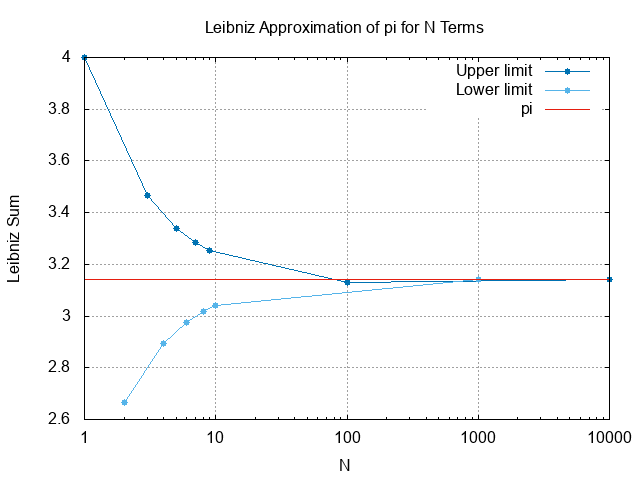
\includegraphics[scale=0.45]{pi_approx_L.png} 
  		\caption{A plot of the Leibniz sum as a function of $N$. The series is an alternating series, and so exhibits a "tunnel" of convergence, emphasized by the upper and lower limit lines. It is clear that this convergence leads to the value of $\pi$. Note that the x-axis is on a log scale.}
  		\label{gr:L}
 	\end{center}
\end{figure}

\begin{figure}[htbp]
 	\begin{center}
 		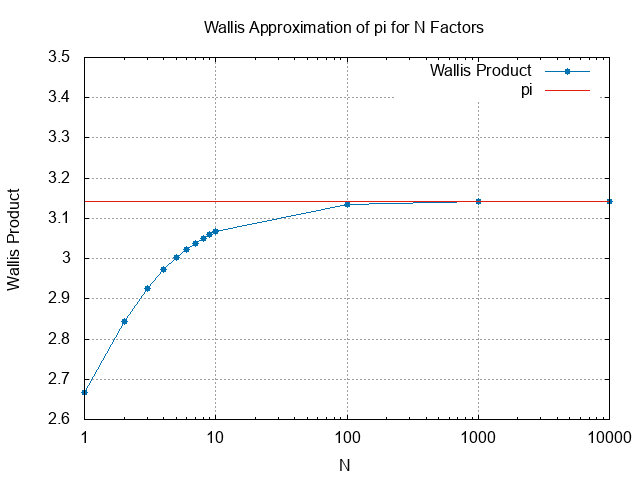
\includegraphics[scale=0.45]{pi_approx_W.png} 
  		\caption{A plot of the Wallis product as a function of $N$. The points are traced to emphasize the track of convergence towards $\pi$, but does not represent the product at any $N$ without a point. Note that the x-axis is on a log scale.}
  		\label{gr:W}
 	\end{center}
\end{figure}

\begin{figure}[htbp]
 	\begin{center}
 		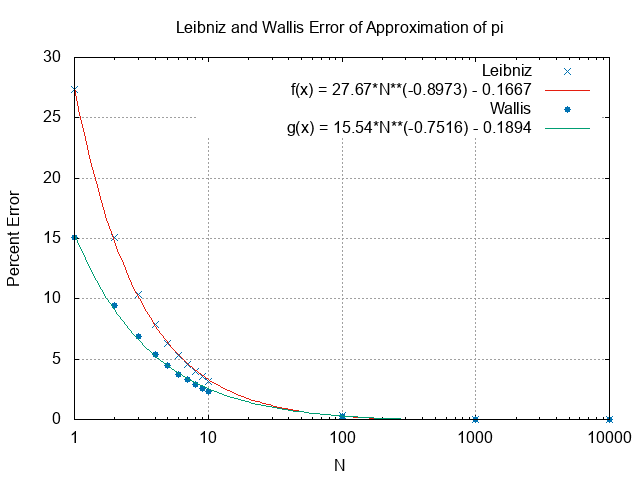
\includegraphics[scale=0.45]{pi_err_fit.png} 
  		\caption{The percent errors of the Leibniz and Wallis approximations for $\pi$. The fits produced have a reduced chi squared of $\chi^2 _{\text{red, L}} = 0.040$ and $\chi^2 _{\text{red, W}} = 0.049$. We can use these fits to determine an estimate for the terms needed to get below a certain percentage of error.}
  		\label{gr:Perr}
 	\end{center}
\end{figure}

We were able to successfully write a program which computed the Leibniz and Wallis approximations for $\pi$ and their percent errors. These values for $N = 1,..., 10, 100, 1000, 10000$ are listed in Table \ref{tbl:pi}. Using these values, we can plot the approximations as a function of $N$ to visualize how the series are converging. From both Figure \ref{gr:L} and \ref{gr:W}, we see a clear convergence towards $\pi$ as $N$ becomes large. To go even further, we can analyze how the percent errors are changing with increasing $N$. Before any fits, we can see that the plots follow something that looks like $x^{-1}$. Then we can use gnuplot to fit the function $f(x) = a x^{-b} + c$ to see how close our guess was. As Figure \ref{gr:Perr} shows, this guess appear to have worked well. 

\section{Discussion}
The figures for the Leibniz series and Wallis approximations show definitive convergence towards $\pi$. From Figure \ref{gr:Perr}, we can see how their rates of convergence compare. The Leibniz approximation begins with larger percent errors than the Wallis formula, but by $N = 10$, they have reached around a common value. From there, they exhibit the same rate of convergence. Since the x-axis in on  log scale, then we can conclude that the rates are extremely slow, needing until about 100 terms to have a percent error less than 1. \\ Mentioned earlier, our guess for a fit function seemed to work, however, if we use these fits to determine how many terms we need to get below a certain percentage of error, the accuracy decreases for large $N$. For example, if we want a percent error less than $\SI{1e-6}{}$, then we calculate
\begin{align}
	\SI{1e-6}{} &< f(N) \\
	\Rightarrow N &> \paren{\frac{\SI{1e-6}{} - c}{a}}^{-1/b} \\
	\rightarrow N_L &> 298 \\
	N_W &> 353 ~.
\end{align}
These are clearly too small, so the model was not exactly correct. So we conclude that the model doesn't fit well for large $N$. So instead, we must realize by looking at Table \ref{tbl:pi} that as $N$ becomes large, the function becomes more inversely proportional to $N$, that is, if $N$ increase by a factor of 10, the percent error decreases by a factor of 10. Using this, we can estimate that we would need $N > \SI{1e8}{}$ terms to have a percent error below $\SI{1e-6}{}$.

\section{Conclusions}
We were able to compute the approximations for $\pi$ using the Leibniz series and Wallis formula for up to $N = 10000$ terms/factors. From the discussions of our results, we found that the rates of convergence were slow and that it would take at least 100 terms to gain a value of $\pi$ with under 1 percent error. And it would take ten times as many terms to decrease the error by 10 from thereon. If we were evaluating these series by hand, trying to calculate the sum or product for 10000 terms would have taken perhaps a year of nonstop calculations, and with likely possibilities of mistakes. A computer program written within a day can compute it within fractions of a second. This shows the power that programming holds for solving physics problems. The only work for us to do thereafter was to analyze the results. And for this assignment, we succeeded in plotting and visualizing the convergence of the two series and comparing their rates of convergence. Using these computational techniques, we can further analyze series in physics and their convergence.

\section*{Acknowledgements}
\setlength{\parindent}{0cm}

\bibliographystyle{aipauth4-1}
\bibliography{bib1}


% \begin{thebibliography}{99}  % the trailing 99 controls some obscure format--just use

% \end{thebibliography}


\end{document}